% Formatted with the FAIR ``fairmeta'' preprint class (arXiv:2505.08762 style).
\documentclass[]{fairmeta}
% Extra packages for this manuscript. fairmeta.cls already loads geometry, graphicx,
% hyperref, natbib, booktabs, bm, microtype, caption, xcolor, etc.
\usepackage{amsmath}
\usepackage{amssymb}
\usepackage{tabularx}
\usepackage{url}
\usepackage{listings}
\usepackage{tikz}
\usetikzlibrary{positioning}
\usepackage{algpseudocode}
\usepackage{chemformula}
\usepackage[version=4]{mhchem}

\definecolor{deepblue}{RGB}{0,0,120}
\definecolor{midgreen}{RGB}{0,120,0}
\definecolor{darkred}{RGB}{120,0,0}
\definecolor{codecolor}{RGB}{240,240,240}

\lstset{
  backgroundcolor=\color{codecolor},
  basicstyle=\footnotesize\ttfamily,
  breaklines=true,
  captionpos=b,
  keepspaces=true,
  columns=flexible,
  tabsize=2,
  frame=single,
  numbers=left,
  numberstyle=\tiny\color{gray},
  keywordstyle=\color{blue},
  commentstyle=\color{darkred},
  stringstyle=\color{midgreen}
}


\title{AI-Driven Design of Fridge-Free Insulin Delivery Patches: An Active Learning Framework Integrating LLMs and Generative Material Discovery}

\author[1]{BioMaterials AI Research Group}
\affiliation[1]{Research Institution, Department of Materials Science and Engineering}

\abstract{This work presents an active learning framework for discovering and optimizing materials for fridge-free insulin delivery patches. The system integrates large language models (LLMs) for scientific literature mining with PSMILES-based generative modeling for material design, creating an iterative discovery pipeline. The implementation employs Ollama~\cite{ollama2023} local LLM infrastructure for literature analysis, a specialized PSMILES generator with conversation memory using LangChain~\cite{chase2022langchain} for material candidate creation, and systematic copolymerization capabilities for structure exploration. The framework identifies diverse material classes through adaptive query generation and polymer structure generation, providing both literature-validated candidates and novel AI-designed materials. This approach aims to accelerate discovery of materials that can maintain insulin stability without refrigeration while enabling controlled transdermal delivery.}

\begin{document}

\maketitle

\section{Introduction}

Maintaining insulin stability without refrigeration represents a critical challenge in diabetes management, particularly in resource-limited settings. Traditional formulations require 2-8°C storage, creating barriers to treatment access. This work addresses designing delivery matrices that maintain insulin biological activity at ambient temperatures through computational discovery methods integrating artificial intelligence approaches.

Insulin degradation involves thermal denaturation through protein unfolding and aggregation, plus chemical degradation via deamidation, oxidation, and fibrillation. Successful materials must simultaneously address these pathways while enabling controlled transdermal delivery through patch formulations.

The approach implemented here utilizes an active learning framework that systematically combines literature knowledge extraction with AI-driven polymer design. The system follows an iterative cycle where literature mining identifies promising material classes, PSMILES-based generative models create polymer candidates, property evaluation assesses material performance, and feedback loops refine subsequent iterations.

The framework addresses key challenges in AI-driven materials discovery: vast literature requiring sophisticated natural language processing, diverse terminology across research domains necessitating robust semantic understanding, and the need for systematic exploration of chemical spaces through generative modeling. The implementation integrates these capabilities through local LLM infrastructure and specialized PSMILES generation systems.

\subsection{Related work}

LLM-based tooling for scientific and engineering tasks is surveyed in recent literature on large models for research~\cite{zhang2025llm} and agentic workflows~\cite{narayana2024agentic}. Our literature stage builds on open scholarly APIs and document representations such as the Semantic Scholar graph~\cite{semantic_scholar_api,cohan2020specter}. Polymer structure generation here uses PSMILES-style repeat units in the spirit of standardized macromolecular line notations~\cite{lin2019bigsmiles}. Planned atomistic evaluation aligns with established GPU-accelerated MD frameworks~\cite{eastman2017openmm}, complementary to the universal interatomic models discussed later~\cite{wood2025uma}.

\section{Active Learning Framework Architecture}

The active learning framework consists of four interconnected components operating in iterative cycles to accelerate material discovery (Figure~\ref{fig:framework}). The integration enables systematic exploration of both literature-validated materials and AI-generated candidates through a closed-loop discovery process.

\begin{figure}[t]
\centering
\resizebox{\linewidth}{!}{%
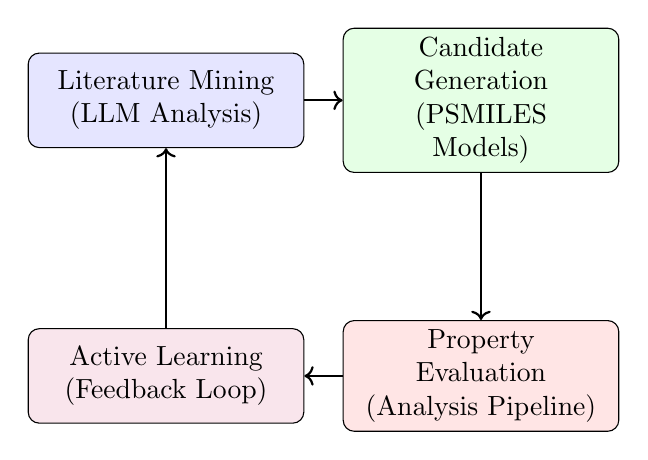
\begin{tikzpicture}[node distance=3cm, auto]
\node (llm) [rectangle, rounded corners, draw, fill=blue!10, minimum width=3.5cm, minimum height=1.2cm, text width=3cm, align=center] {Literature Mining\\(LLM Analysis)};
\node (generate) [rectangle, rounded corners, draw, fill=green!10, minimum width=3.5cm, minimum height=1.2cm, text width=3cm, align=center, right of=llm, xshift=1cm] {Candidate Generation\\(PSMILES Models)};
\node (evaluate) [rectangle, rounded corners, draw, fill=red!10, minimum width=3.5cm, minimum height=1.2cm, text width=3cm, align=center, below of=generate, yshift=-0.5cm] {Property Evaluation\\(Analysis Pipeline)};
\node (feedback) [rectangle, rounded corners, draw, fill=purple!10, minimum width=3.5cm, minimum height=1.2cm, text width=3cm, align=center, below of=llm, yshift=-0.5cm] {Active Learning\\(Feedback Loop)};

\draw[->, thick] (llm.east) -- (generate.west);
\draw[->, thick] (generate.south) -- (evaluate.north);
\draw[->, thick] (evaluate.west) -- (feedback.east);
\draw[->, thick] (feedback.north) -- (llm.south);
\end{tikzpicture}%
}
\caption{Active learning framework integrating literature mining with generative material design. The system iteratively refines material candidates through feedback between LLM analysis and PSMILES-based generation.}
\label{fig:framework}
\end{figure}

The framework operates through iterative cycles where literature mining identifies promising material classes and stabilization mechanisms, PSMILES-based generative models create variants based on these insights, evaluation protocols assess material properties, and feedback loops refine subsequent iterations. This integration enables systematic exploration of chemical space guided by both existing knowledge and AI-generated hypotheses.

% \begin{table}[t]
% \caption{\label{tab:implementation}Active learning framework operational parameters.}
% \begin{ruledtabular}
% \begin{tabular}{ll}
% \textbf{Component} & \textbf{Implementation/Parameters} \\
% \colrule
% Literature Mining & Ollama local LLM, Semantic Scholar API \\
% Query Strategy & Adaptive generation, 8 queries per cycle \\
% Material Extraction & Fast: 1000 tokens, Comprehensive: 3000 tokens \\
% PSMILES Generation & Conversation memory, rule reinforcement \\
% Copolymerization & 4 connection patterns, validation \\
% Feedback Integration & Iterative prompt refinement \\
% Cycle Time & 5-10 minutes per iteration \\
% \end{tabular}
% \end{ruledtabular}
% \end{table}

\begin{figure*}[t]
\begin{lstlisting}[language=Python, caption=Adaptive Query Generation with Active Learning Integration]
def _generate_search_strategy(self, user_request: str, iteration_data: Dict = None) -> Dict:
    # Incorporate feedback from previous iterations if available
    feedback_context = ""
    if iteration_data:
        feedback_context = f"""
PREVIOUS ITERATION INSIGHTS:
- High-performing materials: {iteration_data.get('top_candidates', [])}
- Successful stabilization mechanisms: {iteration_data.get('mechanisms', [])}
- Target properties to optimize: {iteration_data.get('target_properties', [])}
"""
    
    strategy_prompt = f"""# ITERATIVE Material Search Strategy
    
USER REQUEST: "{user_request}"
{feedback_context}

TASK: Generate 8 comprehensive search queries for academic literature.

SEARCH PHILOSOPHY:
- Build on previous iteration insights if provided
- Cast wide net to find diverse materials research
- Include biomaterials, drug delivery, polymer science, protein stabilization
- Use natural language without boolean operators
- Cover multiple application areas for transferable materials
- Focus on thermal stability and controlled release mechanisms

OUTPUT FORMAT (JSON):
{{
  "relevant": true,
  "relevance_score": 10,
  "interpretation": "Search strategy interpretation",
  "search_queries": [
    "thermal stabilization proteins polymers",
    "insulin delivery hydrogel materials",
    "temperature stable protein formulations",
    // ... additional queries
  ],
  "extraction_focus": "Materials with insulin stabilization potential"
}}"""

    response = self.ollama.client.chat(
        model=self.ollama.model_name,
        messages=[{'role': 'user', 'content': strategy_prompt}],
        options={'temperature': 0.3, 'num_predict': 1500}
    )
    
    return self._parse_strategy_response(response['message']['content'])
\end{lstlisting}
\end{figure*}

\section{Literature Mining Component (Milestone 1)}

The literature mining component employs local LLM infrastructure to maintain data privacy while providing natural language processing capabilities. The system processes academic literature through Semantic Scholar API~\cite{lo2020s2orc} integration with Ollama-based analysis for material property extraction.

The literature mining approach dynamically formulates search strategies based on semantic analysis of research objectives and previous iteration results. This replaces static keyword searches with adaptive approaches responding to emerging insights while maintaining focus on insulin delivery applications (see Listing 1). The implementation incorporates feedback from previous iterations to enable progressive refinement of search strategies. The system maintains context about materials and stabilization mechanisms, using this information to guide subsequent literature exploration toward promising material classes. The system can generate a comprehensive list of materials derived from the literature. The user can then take one candidate and input that to the next stage of the workflow, which is on generating the material candidate and modifying it further. While this part is only manual for now, automation is planned as part of the final milestone.

Building upon this adaptive query generation foundation, the processing pipeline implements a multi-stage approach that maximizes both coverage and depth through sequential refinement guided by active learning principles. Each iteration builds upon previous results to explore related chemical spaces systematically, as demonstrated in the iterative literature processing implementation (Listing 2). This processing integrates active learning feedback to progressively focus searches on promising material classes while maintaining exploration of adjacent chemical spaces, enabling systematic discovery of both known materials and variations.

\begin{figure*}[t]
\begin{lstlisting}[language=Python, caption=Iterative Literature Processing with Feedback Integration]
def search_papers_with_feedback(self, topic: str, iteration_context: Dict = None, 
                               max_results: int = 20) -> List[Dict]:
    # Adjust search strategy based on iteration context
    if iteration_context and iteration_context.get('successful_materials'):
        # Focus on related materials and mechanisms
        related_queries = self._generate_related_material_queries(
            iteration_context['successful_materials']
        )
        topic = f"{topic} OR {' OR '.join(related_queries)}"
    
    year_filter = "2020-" if iteration_context and iteration_context.get('recent_focus') else None
    
    # Strategy 1: Target high-impact papers with iteration-specific focus
    results = self.search_papers(
        query=topic,
        limit=max_results,
        year_range=year_filter,
        min_citation_count=5 if iteration_context else 1
    )
    papers = self._process_search_results(results)
    
    # Strategy 2: Expand to explore adjacent chemical spaces
    if len(papers) < max_results // 2 and iteration_context:
        adjacent_topics = self._identify_adjacent_topics(iteration_context)
        for adj_topic in adjacent_topics:
            results = self.search_papers(
                query=adj_topic,
                limit=max_results // len(adjacent_topics),
                year_range=year_filter
            )
            papers.extend(self._process_search_results(results))
    
    return papers[:max_results]
\end{lstlisting}
\end{figure*}

\section{Candidate Generation Component (Milestone 2)}

The candidate generation component implements a specialized PSMILES (Polymer SMILES) generator with conversation memory and systematic copolymerization capabilities. PSMILES notation, an extension of SMILES for polymer representation~\cite{sokolova2021molecular}, enables systematic computational manipulation of polymer structures. This component creates polymer structures based on insights from literature mining while exploring chemical space through rule-based generation and structural modifications.

The PSMILES generator employs large language models with enhanced conversation memory using LangChain's ConversationBufferWindowMemory~\cite{chase2022langchain} and rule reinforcement mechanisms to ensure chemically valid polymer structure generation. The system maintains adherence to PSMILES notation while incorporating domain-specific knowledge for insulin delivery applications (Listing 3). The generator maintains comprehensive rule sets ensuring chemical validity while providing flexibility for structure generation, with conversation memory enabling progressive refinement of generated structures based on previous interactions and feedback.

\begin{figure*}[t]
\begin{lstlisting}[language=Python, caption=PSMILES Generator Core Implementation with Conversation Memory]
class PSMILESGenerator:
    def __init__(self, ollama_model: str = "llama3.2", ollama_host: str = "http://localhost:11434"):
        self.llm = Ollama(
            model=ollama_model,
            base_url=ollama_host,
            temperature=0.1  # Low temperature for consistent chemical generation
        )
        
        # Initialize conversation memory to maintain context
        self.memory = ConversationBufferWindowMemory(
            k=10,  # Keep last 10 exchanges to maintain recent context
            return_messages=True,
            memory_key="chat_history"
        )
        
        # Load PSMILES rules and examples
        self.psmiles_rules = self._get_psmiles_rules()
        self.psmiles_examples = self._get_psmiles_examples()
        
        # Track conversation turns for rule reinforcement
        self.conversation_count = 0
        self.rule_reinforcement_interval = 5  # Reinforce rules every 5 interactions
    
    def _get_psmiles_rules(self) -> str:
        return """
CRITICAL PSMILES (Polymer SMILES) RULES - FOLLOW EXACTLY:

1. **NO SPACES**: PSMILES strings NEVER contain spaces
2. **NO HYPHENS**: PSMILES strings NEVER contain hyphens (-)
3. **ATOMS**: Use atomic symbols (C, N, O, S, F, Cl, Br, etc.)
4. **BONDS**: Single bonds: atoms next to each other (CC), Double bonds: = symbol (C=C)
5. **BRANCHES**: Use round brackets ()
6. **CONNECTION POINTS**: Use [*] for polymer connections - CRITICAL!

MANDATORY CONNECTION POINT RULES:
- PSMILES represents polymer REPEAT UNITS with exactly 2 connection points
- MUST have exactly 2 [*] symbols - NEVER 0, 1, 3, 4, or more!
- ALL PSMILES strings MUST have exactly 2 [*] symbols to specify connection points
- [*] shows exactly WHERE the polymer unit connects to adjacent units

CRITICAL EXAMPLES:
- PEG (ether linkage): [*]OCC[*] (connects through marked positions)
- Ethylene: [*]CC[*] (simple alkyl chain)
- Meta-phenylene: [*]C(C=C1)=CC([*])=C1 (aromatic with marked positions)
"""
\end{lstlisting}
\end{figure*}

To ensure reliability for common polymer requests, the system implements comprehensive direct mapping and fallback mechanisms that guarantee correct PSMILES generation for well-known materials while maintaining the ability to generate structures (Listing 4). These mechanisms provide robust fallback options that ensure the system can handle both standard polymer requests and generation tasks.

\begin{figure*}[t]
\begin{lstlisting}[language=Python, caption=Direct Mapping and Fallback Mechanisms for Reliable PSMILES Generation]
def _direct_psmiles_mapping(self, request: str) -> Optional[Dict]:
    """Direct mapping for common polymer requests to ensure correct PSMILES."""
    request_lower = request.lower()
    
    # Comprehensive mapping with correct PSMILES - ALL must have exactly 2 [*] symbols
    direct_mapping = {
        'peg': {
            'psmiles': '[*]OCC[*]',
            'explanation': 'This represents the polyethylene glycol repeat unit -O-CH2-CH2- with connection points marked by [*]'
        },
        'polyethylene glycol': {
            'psmiles': '[*]OCC[*]',
            'explanation': 'This represents the polyethylene glycol repeat unit -O-CH2-CH2- with connection points marked by [*]'
        },
        'polyethylene': {
            'psmiles': '[*]CC[*]',
            'explanation': 'This represents the ethylene repeat unit -CH2-CH2- with exactly 2 connection points'
        },
        'polystyrene': {
            'psmiles': '[*]CC([*])C1=CC=CC=C1',
            'explanation': 'This represents the styrene repeat unit with benzene ring and exactly 2 connection points'
        },
        'polypropylene': {
            'psmiles': '[*]CC([*])C',
            'explanation': 'This represents the propylene repeat unit -CH2-CH(CH3)- with exactly 2 connection points'
        },
        'nylon': {
            'psmiles': '[*]NC(=O)CCCCC[*]',
            'explanation': 'This represents a nylon repeat unit with exactly 2 connection points'
        },
        'polyamide': {
            'psmiles': '[*]NC(=O)C[*]',
            'explanation': 'This represents a polyamide repeat unit with exactly 2 connection points'
        }
    }
    
    # Check for exact matches first, then partial matches
    for key, info in direct_mapping.items():
        if key == request_lower or key in request_lower:
            return info
    
    return None

def _fallback_psmiles_extraction(self, request: str, response: str) -> Dict:
    """Enhanced fallback mechanism for PSMILES extraction."""
    request_lower = request.lower()
    
    # Extended fallback mapping for additional polymer types
    fallback_mapping = {
        'polyester': '[*]OC(=O)C[*]',
        'pet': '[*]OC(=O)C1=CC=C(C[*])C=C1',
        'pvp': '[*]CC([*])C1=CN(C)C=C1',
        'pva': '[*]CC([*])O',
        'pmma': '[*]CC([*])(C)C(=O)OC',
        'meta phenylene': '[*]C1=CC([*])=CC=C1',
        'para phenylene': '[*]C1=CC=C([*])C=C1',
        'ortho phenylene': '[*]C1=C([*])C=CC=C1'
    }
    
    for keyword, psmiles in fallback_mapping.items():
        if keyword in request_lower:
            return {
                'psmiles': psmiles,
                'pattern': 'fallback_mapping',
                'note': f'Used fallback mapping for {keyword}'
            }
    
    return {'psmiles': None, 'pattern': None}
\end{lstlisting}
\end{figure*}

The material generation approach extends beyond simple structure generation to include systematic copolymerization capabilities that enable exploration of complex polymer architectures through controlled combination of different monomer units. This approach creates materials by combining beneficial properties from different polymer components (Listing 5). The copolymerization system enables systematic exploration of material properties by combining different functional groups with base polymer structures, creating libraries of related materials with varying properties for systematic evaluation in the active learning cycle.

\begin{figure*}[t]
\begin{lstlisting}[language=Python, caption=Copolymerization Implementation for Novel Material Design]
def handle_copolymerization_request(message: str, session_id: str) -> Dict:
    """Handle copolymerization requests for material design."""
    # Extract second PSMILES and connection pattern
    psmiles_pattern = r'(\[[^\]]*\][A-Za-z0-9\[\]\(\)\=\#\*\-\+\\\/]*|\b[A-Za-z0-9\[\]\(\)\=\#\*\-\+\\\/]{5,})'
    potential_psmiles = re.findall(psmiles_pattern, message)
    
    if not potential_psmiles:
        return {
            'type': 'error',
            'message': 'Please provide the second PSMILES string for copolymerization.',
            'suggestion': 'Example: "copolymerize with [*]CC(=O)[*] using pattern [1,1]"'
        }
    
    second_psmiles = potential_psmiles[0]
    
    # Extract connection pattern - critical for material design
    pattern_match = re.search(r'\[(\d+),\s*(\d+)\]', message)
    if pattern_match:
        connection_pattern = [int(pattern_match.group(1)), int(pattern_match.group(2))]
    else:
        connection_pattern = [1, 1]  # default alternating pattern
    
    result = psmiles_processor.perform_copolymerization(
        session_id, psmiles_index, second_psmiles, connection_pattern
    )
    
    return {
        'type': 'psmiles_copolymer',
        'copolymer_result': result,
        'svg_content': result.get('svg_content', ''),
        'timestamp': datetime.now().isoformat()
    }

def _generate_functional_group_variants() -> Dict[str, str]:
    """Generate functional group variants for systematic material design."""
    functional_group_fragments = {
        'hydroxyl': '[*]C(O)[*]',        # Carbon with -OH attached
        'carboxyl': '[*]C(=O)O[*]',      # Carboxyl group for ionic interactions
        'amine': '[*]C(N)[*]',           # Carbon with -NH2 for hydrogen bonding
        'amide': '[*]C(=O)N[*]',         # Amide group for protein interaction
        'carbonyl': '[*]C(=O)[*]',       # Carbonyl group for specific binding
        'ester': '[*]C(=O)OC[*]',        # Ester linkage for degradability
        'ether': '[*]COC[*]',            # Ether linkage for flexibility
        'alkene': '[*]C=C[*]',           # Alkene for crosslinking potential
        'alkyne': '[*]C#C[*]',           # Alkyne for click chemistry
        'haloalkane': '[*]C(Cl)[*]',     # Halogen for specific interactions
        'aromatic': '[*]c1ccc(cc1)[*]'   # Aromatic for pi-pi interactions
    }
    return functional_group_fragments
\end{lstlisting}
\end{figure*}

To ensure comprehensive exploration of chemical space, the system additionally implements random material generation capabilities that create diverse polymer candidates for screening and evaluation (Listing 6). This random generation capability complements the targeted copolymerization approach by providing systematic exploration of chemical combinations that might not be immediately obvious from literature insights, thereby expanding the breadth of material candidates for evaluation.

\begin{figure*}[t]
\begin{lstlisting}[language=Python, caption=Random PSMILES Generation for Chemical Space Exploration]
def _generate_random_psmiles() -> str:
    """Generate a random PSMILES string for copolymerization and exploration."""
    import random
    
    # List of common polymer building blocks for systematic exploration
    random_blocks = [
        "[*]CC(=O)[*]",           # Ketone functionality
        "[*]C(=O)O[*]",           # Carboxyl functionality
        "[*]NC(=O)[*]",           # Amide functionality
        "[*]c1ccc(cc1)[*]",       # Aromatic functionality
        "[*]CC(C)[*]",            # Branched alkyl structure
        "[*]C(=O)N[*]",           # Alternative amide orientation
        "[*]OC(=O)[*]",           # Ester functionality
        "[*]CCOC(=O)[*]",         # Extended ester structure
        "[*]NC(C)C(=O)[*]",       # Amino acid-like structure
        "[*]C(=O)CCC(=O)[*]",     # Diketone structure for crosslinking
        "[*]C(O)C[*]",            # Hydroxyl functionality
        "[*]C(F)(F)[*]",          # Fluorinated structure for unique properties
        "[*]SC[*]",               # Sulfur-containing structure
        "[*]C(=S)[*]"             # Thiocarbonyl functionality
    ]
    
    return random.choice(random_blocks)

def generate_material_library(self, base_insights: Dict, library_size: int = 20) -> List[Dict]:
    """Generate a library of material candidates for systematic evaluation."""
    material_library = []
    
    # Generate systematic variations
    for i in range(library_size):
        # Combine random blocks for novel materials
        base_block = self._generate_random_psmiles()
        functional_block = random.choice(list(self._generate_functional_group_variants().values()))
        
        # Create copolymer candidate
        connection_patterns = [[0, 1], [1, 0], [0, 0], [1, 1]]
        pattern = random.choice(connection_patterns)
        
        material_candidate = {
            'base_psmiles': base_block,
            'functional_psmiles': functional_block,
            'connection_pattern': pattern,
            'generation_method': 'systematic_exploration',
            'candidate_id': f'MAT_{i:03d}',
            'predicted_properties': self._predict_basic_properties(base_block, functional_block)
        }
        
        material_library.append(material_candidate)
    
    return material_library
\end{lstlisting}
\end{figure*}

\section{Property Evaluation Component (Analysis Pipeline)}

The property evaluation component processes both literature-derived and AI-generated materials through systematic assessment protocols. This analysis enables comparison between known materials and candidates generated through PSMILES-based design. Currently implemented as basic property scoring with plans for advanced computational evaluation (Listing 7), the evaluation system provides structured feedback enabling iterative refinement of both literature mining strategies and generative model parameters. This active learning approach progressively improves material discovery through systematic integration of evaluation results.

\begin{figure*}[t]
\begin{lstlisting}[language=Python, caption=Material Property Evaluation Framework]
def evaluate_material_candidates(self, literature_materials: List[Dict], 
                               generated_materials: List[Dict]) -> Dict:
    """
    Evaluate both literature-derived and AI-generated materials,
    providing feedback for next iteration.
    """
    
    all_candidates = literature_materials + generated_materials
    evaluation_results = []
    
    for material in all_candidates:
        # Extract or predict key properties
        properties = self._assess_material_properties(material)
        
        # Score based on insulin delivery criteria
        score = self._calculate_insulin_delivery_score(properties)
        
        evaluation_results.append({
            'material': material,
            'properties': properties,
            'score': score,
            'source': 'literature' if material in literature_materials else 'generated'
        })
    
    # Rank candidates and identify top performers
    ranked_candidates = sorted(evaluation_results, key=lambda x: x['score'], reverse=True)
    
    # Generate feedback for next iteration
    feedback = self._generate_iteration_feedback(ranked_candidates)
    
    return {
        'ranked_candidates': ranked_candidates,
        'top_performers': ranked_candidates[:10],
        'iteration_feedback': feedback,
        'insights': self._extract_design_insights(ranked_candidates)
    }

def _calculate_insulin_delivery_score(self, properties: Dict) -> float:
    """Calculate composite score for insulin delivery applications."""
    # Basic scoring based on available properties
    thermal_stability_score = properties.get('thermal_stability_score', 0.5)
    biocompatibility_score = properties.get('biocompatibility_score', 0.5)
    release_control_score = properties.get('release_control_score', 0.5)
    
    # Weighted combination for insulin delivery
    weights = {'thermal': 0.4, 'biocompat': 0.3, 'release': 0.3}
    
    composite_score = (
        weights['thermal'] * thermal_stability_score +
        weights['biocompat'] * biocompatibility_score +
        weights['release'] * release_control_score
    )
    
    return composite_score
\end{lstlisting}
\end{figure*}

\section{Active Learning Component (Feedback Loop)}

The active learning component implements feedback mechanisms that integrate evaluation results into subsequent iterations of both literature mining and material generation. This creates an active learning system where each iteration builds upon previous discoveries (Listing 8). The system maintains traceability linking generated materials to literature sources and evaluation results, enabling systematic understanding of structure-property relationships while supporting reproducible research practices through citation management.

\begin{figure*}[t]
\begin{lstlisting}[language=Python, caption=Active Learning Feedback Integration]
def _generate_iteration_feedback(self, ranked_candidates: List[Dict]) -> Dict:
    """Generate structured feedback for next active learning iteration."""
    
    top_materials = ranked_candidates[:5]
    bottom_materials = ranked_candidates[-5:]
    
    # Identify successful patterns
    successful_features = self._analyze_successful_features(top_materials)
    problematic_features = self._analyze_problematic_features(bottom_materials)
    
    return {
        'successful_materials': [m['material'] for m in top_materials],
        'beneficial_features': successful_features,
        'avoid_features': problematic_features,
        'target_properties': self._refine_target_properties(top_materials),
        'next_iteration_focus': self._determine_next_focus(ranked_candidates),
        'psmiles_generation_hints': self._extract_psmiles_patterns(top_materials)
    }

def _extract_psmiles_patterns(self, top_materials: List[Dict]) -> Dict:
    """Extract successful PSMILES patterns for next generation cycle."""
    successful_patterns = {
        'functional_groups': [],
        'backbone_structures': [],
        'connection_strategies': [],
        'molecular_motifs': []
    }
    
    for material_result in top_materials:
        material = material_result['material']
        if 'psmiles' in material:
            psmiles = material['psmiles']
            
            # Extract functional groups
            functional_groups = self._identify_functional_groups(psmiles)
            successful_patterns['functional_groups'].extend(functional_groups)
            
            # Extract backbone patterns
            backbone = self._extract_backbone_pattern(psmiles)
            if backbone:
                successful_patterns['backbone_structures'].append(backbone)
    
    return successful_patterns

def update_next_iteration_parameters(self, feedback: Dict) -> Dict:
    """Update parameters for next iteration based on feedback."""
    next_params = {
        'literature_search_focus': feedback.get('next_iteration_focus', 'general'),
        'psmiles_generation_bias': feedback.get('psmiles_generation_hints', {}),
        'target_properties': feedback.get('target_properties', {}),
        'avoid_features': feedback.get('avoid_features', []),
        'beneficial_features': feedback.get('beneficial_features', [])
    }
    
    return next_params
\end{lstlisting}
\end{figure*}

\section{Work-in-progress: MD Simulation and Advanced Evaluation (TBD)}

Future development phases will integrate advanced computational evaluation capabilities to replace the current basic property scoring system. These planned enhancements will provide quantitative validation of material performance for insulin delivery applications.

\subsection{Molecular Dynamics Simulation Integration (Planned)}

The framework will incorporate molecular dynamics simulations using Meta's Universal Model for Atoms (UMA) force field~\cite{wood2025uma} for rapid evaluation of materials without traditional parameterization bottlenecks. The PSMILES-generated candidates will serve as direct inputs for MD simulations evaluating thermal stability mechanisms, insulin-material interactions, and release kinetics at atomic resolution.

The planned MD integration will employ the Atomic Simulation Environment (ASE)~\cite{larsen2017atomic} for interfacing with UMA, enabling simulation workflows that evaluate critical properties including thermal stability through high-temperature NPT simulations, insulin protection through protein secondary structure analysis, water penetration through diffusion coefficient calculations, and release kinetics through steered MD with potential of mean force calculations.

\subsection{Machine Learning Property Prediction (Planned)}

Machine learning integration represents a natural extension where structure-property relationships identified through active learning cycles will inform predictive models for rapid candidate screening. The comprehensive database will serve as training data for specialized models predicting insulin stabilization properties directly from PSMILES representations.

The planned implementation will incorporate graph neural networks trained specifically on polymer structures for insulin delivery applications, reinforcement learning approaches enabling optimization of generative models based on evaluation feedback, and multi-objective optimization capabilities balancing competing requirements including thermal stability, biocompatibility, mechanical properties, and manufacturing feasibility.

\subsection{Experimental Validation Protocols (Planned)}

The framework provides a systematic foundation for clinical translation through comprehensive material characterization and traceability to literature sources. Future development will incorporate experimental validation protocols integrating with laboratory workflows for rapid candidate screening and automated synthesis planning based on PSMILES representations.

\subsection{Implementation status}

The running stack requires a live \textbf{Ollama} server for literature extraction (no keyword-only substitute). MD evaluation and the autonomous discovery loop require \textbf{OpenMM} and the insulin PDB (no empty placeholder feedback). Mutation, when enabled, requires installed psmiles/mutation dependencies.

\section{Conclusions}

This work implemented and evaluated an active learning framework integrating LLM-based literature mining with PSMILES-based generative material design for insulin delivery applications. The system combines literature knowledge extraction with systematic generation of material candidates through iterative refinement cycles.

The PSMILES generator component employs conversation memory and systematic copolymerization capabilities to create chemically valid polymer structures while exploring diverse chemical spaces. The implementation achieves generation of polymer candidates with proper PSMILES notation, comprehensive fallback mechanisms for known materials, and systematic exploration capabilities through random generation and functional group combination.

The framework identifies promising material classes through adaptive query generation while systematically exploring chemical variations through PSMILES-based polymer design. Active learning integration enables progressive refinement of both literature mining strategies and generative model parameters, creating co-evolution between knowledge extraction and material discovery.

The modular architecture provides a foundation for integration with advanced computational methods including molecular dynamics simulations and quantum mechanical calculations. The PSMILES representation enables direct translation of AI-generated designs to computational chemistry workflows while maintaining comprehensive traceability through citation management systems.

Future development will focus on implementing the planned MD simulation capabilities using Meta's UMA force field and machine learning property prediction models. The current implementation provides essential infrastructure for these advanced capabilities while delivering immediate value through systematic integration of literature mining and PSMILES-based material generation for insulin delivery applications.

\section{Acknowledgments}

We acknowledge the open-source communities that developed the Ollama framework, Semantic Scholar API, LangChain, and Flask web framework, which enabled the implementation of this active learning system. We also thank the materials science research community for providing the foundational literature that makes AI-driven material discovery possible.

\bibliographystyle{plainnat}
\bibliography{../paper/references}

\end{document}